\section{Soluci\'on}
	\setlength{\parindent}{1em}
	\setlength{\parskip}{10pt}
	\subsection{Protocolo IP}
		\begin{figure}[h]
			\centering		
			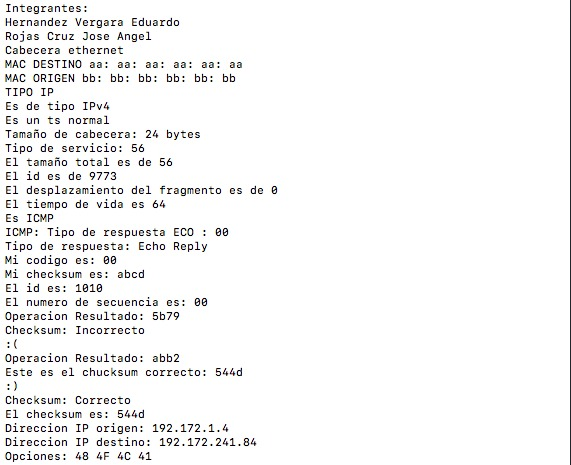
\includegraphics[width=\textwidth]{Ejercicio1}
			\caption{Una trama IP con opciones -ICMP- se imprimen las opciones en hexadecimal}
		\end{figure}
	\begin{figure}[h]
			\centering		
			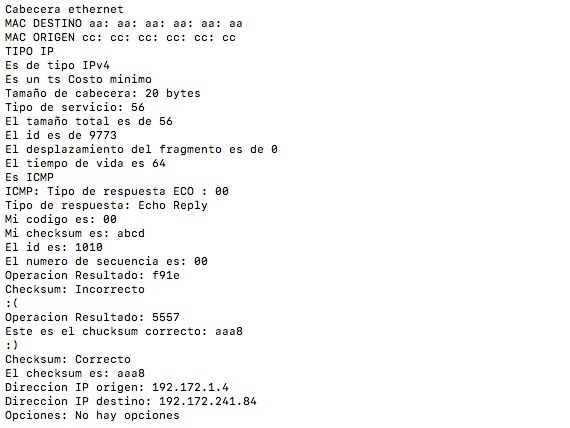
\includegraphics[width=\textwidth]{Ejercicio2}
			\caption{Una trama IP de costo mínimo y se imprime TTL}
		\end{figure}
		\begin{figure}[h]
			\centering		
			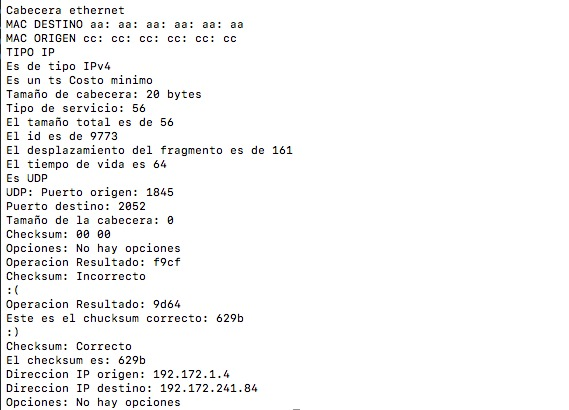
\includegraphics[width=\textwidth]{Ejercicio3}
			\caption{Una trama UDP cuyo encapsulado IP no tiene opciones y se devuelve el valor del offset en decimal}
		\end{figure}
		\begin{figure}[h]
			\centering		
			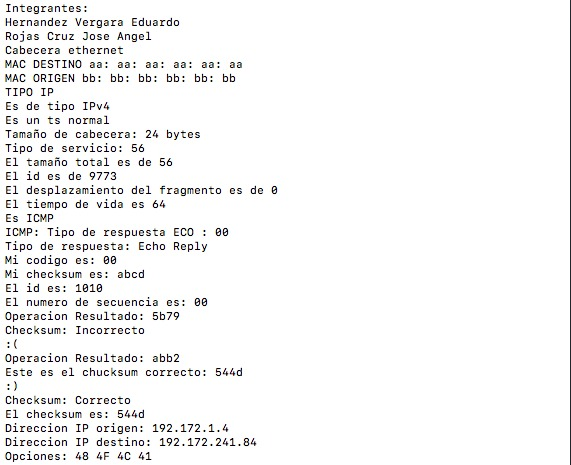
\includegraphics[width=\textwidth]{Ejercicio1}
			\caption{Verificar el checksum de las tramas IP, en caso de que este correcto imprimir :) en caso de que sea incorrecto :( e imprimir el checksum correcto.}
		\end{figure}
	\clearpage
\subsection{Protocolo TCP}
Colocar el c\'odigo correspondiente para la construccion de la pseudocabecera TCP. Y resultados de su ejecuci\'on para una trama con el Checksum correcto y otra con el checksum incorrecto.
		\begin{figure}[h]
			\centering		
			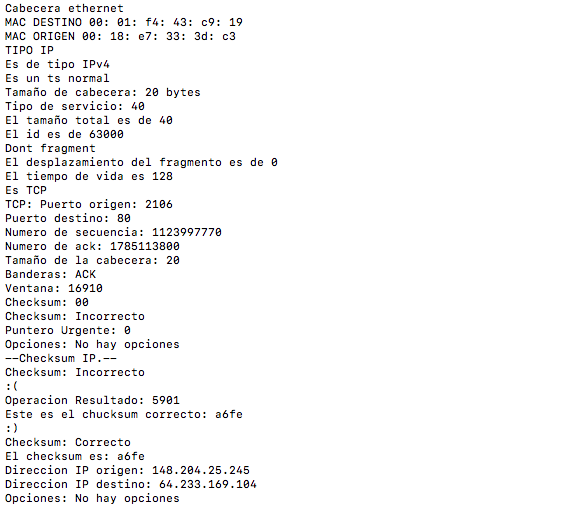
\includegraphics[width=\textwidth]{tcp1}
			\caption{Ejemplo 1}
		\end{figure}
	\begin{figure}[h]
			\centering		
			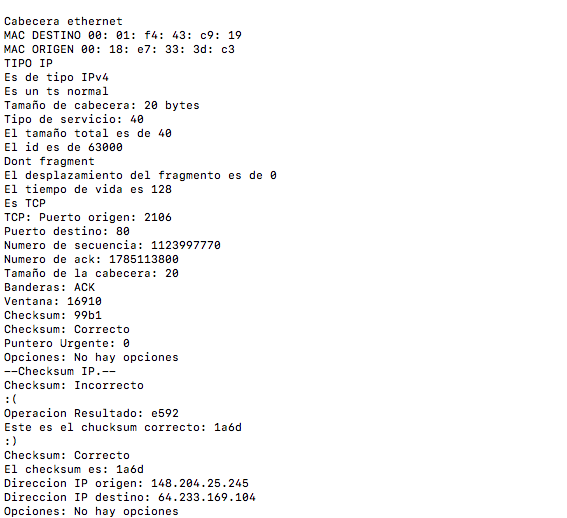
\includegraphics[width=\textwidth]{tcp2}
			\caption{Ejemplo 2}
		\end{figure}
\clearpage
\subsection{Protocolo UDP}
Para la implementaci\'on de este an\'alizador se imprimen solamente los campos 
Poner el c\'odigo correspondiente y la s\'alida para dos tramas ejemplo. 
		\begin{figure}[h]
			\centering		
			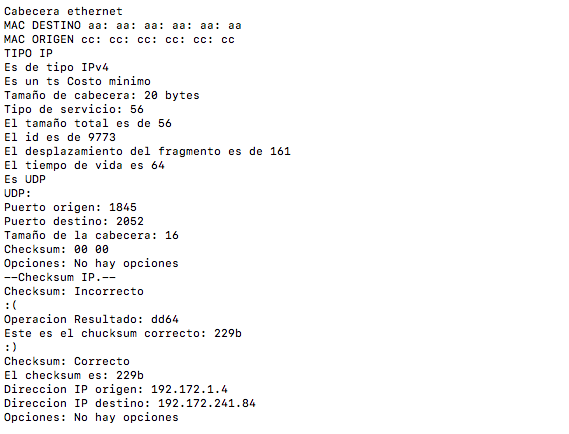
\includegraphics[width=\textwidth]{udp1}
			\caption{Ejemplo 1}
		\end{figure}
	\begin{figure}[h]
			\centering		
			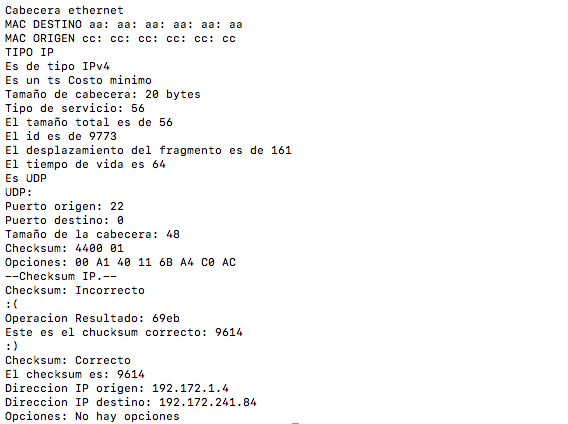
\includegraphics[width=\textwidth]{udp2}
			\caption{Ejemplo 2}
		\end{figure}
\clearpage